\icode{E-MD-MU-L3-261119-001}
（多选）
如图所示，\(a\)、\(b\)、\(c\)三个物块的质量分别为\(m\)、\(2m\)、\(m\)，物块\(a\)、\(b\)通过水平轻绳相连后放水平面上，物块\(c\)放在\(b\)上。现用水平恒力\(F\)作用在\(a\)上，使三个物块一起水平向右做与加速运动。各接触面间的动摩擦因数均为\(\mu\)重力加速度大小为\(g\)。下列说法正确的是\paren[]

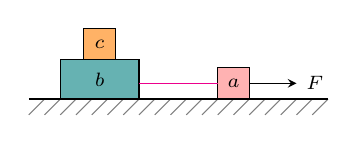
\begin{tikzpicture}[>=stealth,font=\scriptsize]
	\draw[fill=teal!60] (0,0) rectangle(1,.5)node[midway]{\(b\)};
    \draw[fill=orange!60] (.3,.5)rectangle (.7,.9)node[midway]{\(c\)};
    \draw[fill=red!30] (2,0) rectangle(2.4,.4)node[midway]{\(a\)};
	\draw[magenta] (1,.2)--(2,.2);
	\draw[->] (2.4,.2)--(3,.2)node[right]{\(F\)};
	\foreach \x in {-.4,-.2,...,3.2}
		\draw[gray] (\x,-.2)--++(.2,.2);
	\draw[thick] (-.4,0)--(3.4,0);
\end{tikzpicture}
\begin{choices}
	\item 物块\(c\)受到的摩擦力大小为\(2\mu mg\)
	\item 绳子拉力大小等于\(\frac{3}{4}F\)
	\item 物块\(c\)受到的摩擦力大小为\(\frac{1}{4}F\)
	\item 剪断轻绳后，在物块\(b\)向右运动的过程中，物块\(c\)受到的摩擦力大小为\(\mu mg\)
\end{choices}
\begin{answer}
	BCD\qquad 提示：
\end{answer}